% Generated by thesis/ch7/exp1/make_figures.py -- do not edit by hand.
\begin{figure}[tbp]
  \centering
  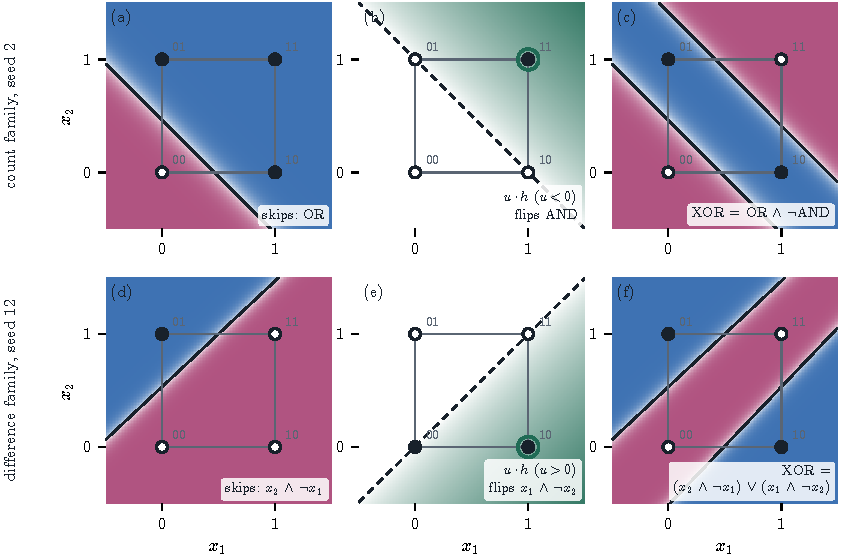
\includegraphics[width=\textwidth,height=0.8\textheight,keepaspectratio]{figures/ch7/xor-gates.pdf}
  \caption{XOR: the gates of each family, count family (a--c) and difference family (d--f). Left: the skip connections alone; middle: the hidden unit's contribution $u\cdot h$ (green: active, darker for larger $|u h|$; dashed: its fold; ringed points: the inputs whose sign it flips); right: the composed score. Shading: blue where the score is positive, magenta where it is negative, pale near 0; solid line: where it is 0. Filled points: inputs where the panel's quantity is positive (middle: where the hidden unit is active).}
  \label{fig:ch7-xor-gates}
\end{figure}
